\documentclass[a4paper,11pt]{article}

% set length of paper. put 'true' before unit like 31mm = 30truemm.
\usepackage[top=25truemm,bottom=25truemm,left=23truemm,right=23truemm]{geometry}
% set font to 'Times'
\usepackage{newtxtext,newtxmath}
% multi column
\usepackage{multicol}
\usepackage{color}
\usepackage[dvipdfmx]{graphics}
\usepackage{amsmath,amssymb}
\usepackage{bm} % italic bold (vector)
\usepackage{authblk} % author
\usepackage{fancyhdr} % header and footer
\usepackage{graphicx}
\usepackage{ascmac}
\usepackage{caption}
\usepackage{tikz}
\usepackage{here}
\usepackage{wrapfig} % 画像にテキストを回り込ませる
\usepackage{listings} % source code
\usepackage[version=3]{mhchem} %chemical equatio
\usepackage{titlesec} % relates to section

% settings of section and subsection
%\makeatletter
%\def\section{\@startsection {section}{1}{\z@}{0.1ex plus 2ex minus -.2ex}{0.1ex plus .2ex}{\normalsize\textbf}}
%\def\subsection{\@startsection {subsection}{1}{\z@}{0.1ex plus 2ex minus -.2ex}{0.1ex plus .2ex}{\normalsize\textbf}}
%\makeatother
%\pagestyle{empty}
%
%\setlength{\textwidth}{\fullwidth}
%\setlength{\texthight}{40\baselineskip}
%\addtolength{\texthight}{\topskip}
%\setlength{voffset}{-0.55in}
%
% キャプションの設定
\captionsetup[figure]{format=plain, labelformat=simple, labelsep=space, font=footnotesize}
\captionsetup[table]{format=plain, labelformat=simple, labelsep=space, font=footnotesize}
\renewcommand{\figurename}{Figure}
\renewcommand{\tablename}{Table}
%
% setting of source code
\lstset{
    basicstyle={\scriptsize\ttfamily},
    breakindent = 30pt,
    stringstyle={\scriptsize\ttfamily},
    basicstyle={\ttfamily},
  identifierstyle={\small},
  commentstyle={\smallitshape},
  keywordstyle={\small\bfseries},
  ndkeywordstyle={\small},
  stringstyle={\small\ttfamily},
  frame={tb},
  breaklines=true,
  columns=[l]{fullflexible},
  numbers=left,
  xrightmargin=0zw,
  xleftmargin=3zw,
  numberstyle={\scriptsize},
  stepnumber=1,
  numbersep=1zw,
  keepspaces=true,
  lineskip=-0.5ex,
}
% document
\begin{document}
% START DOCUMENT
%
% HEADER
\begin{center}
  % title, author
  {\fontsize{16pt}{16pt}\selectfont Numerical Analysis assignment No. 6\\}
  \vspace{16pt}
  \fontsize{10.5pt}{12pt}\selectfont
  B6TB1505 Daichi HAYASHI (Ohnishi Lab.)\\
  \vspace{10.5pt}
  \today \\
  \vspace{-2mm}
\end{center}

\section{Von–Neumann analysis of Lax–Wendroff scheme.}
The result is shown below as Figure 1–3.

\begin{figure}[H]
	\centering
	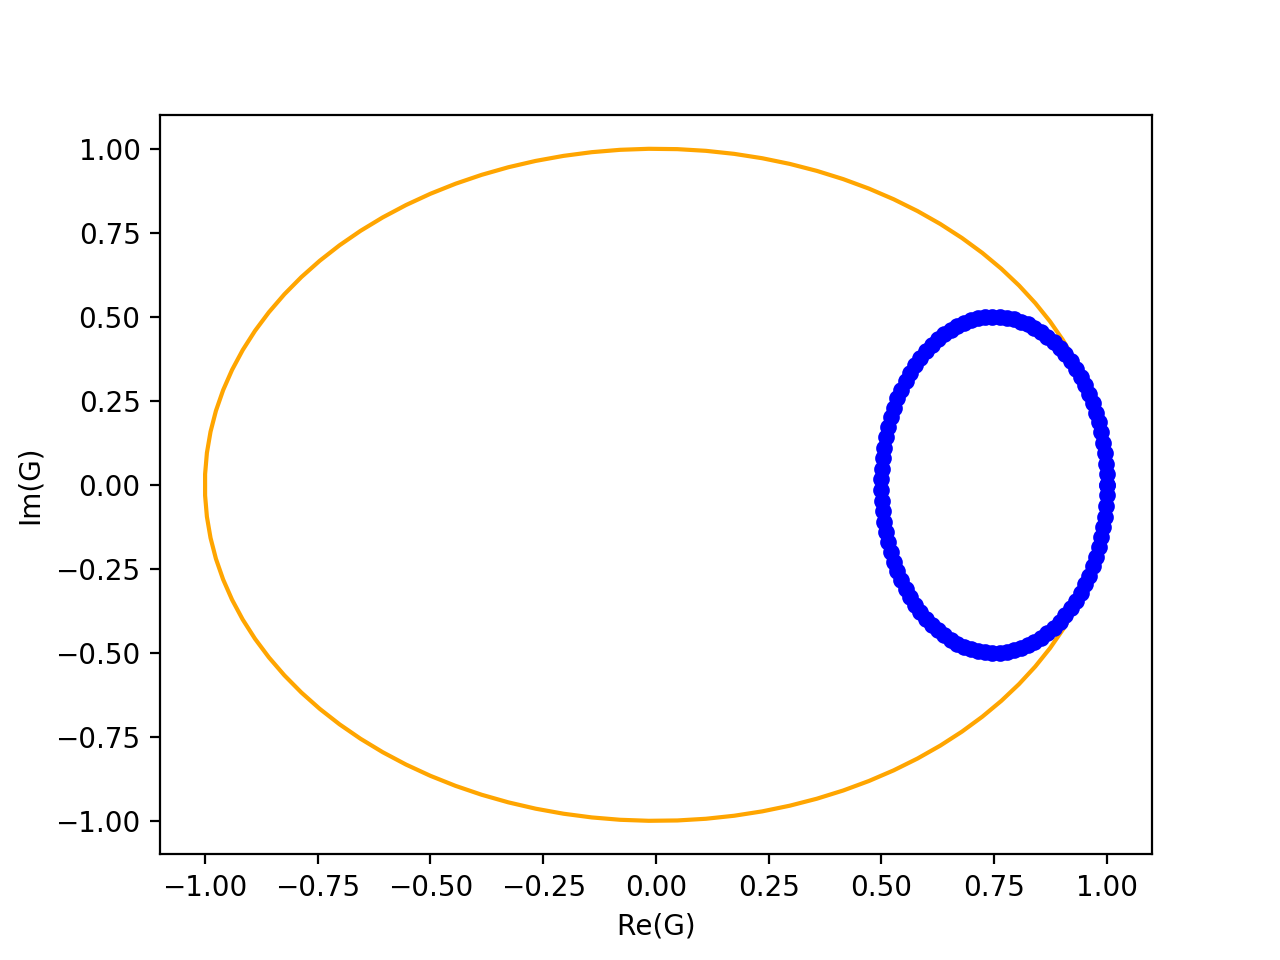
\includegraphics[width=10cm]{fig/vn05.png}
	\caption{Von–Neumann analysis with convection number = 0.5.} 
\end{figure}

\begin{figure}[H]
	\centering
	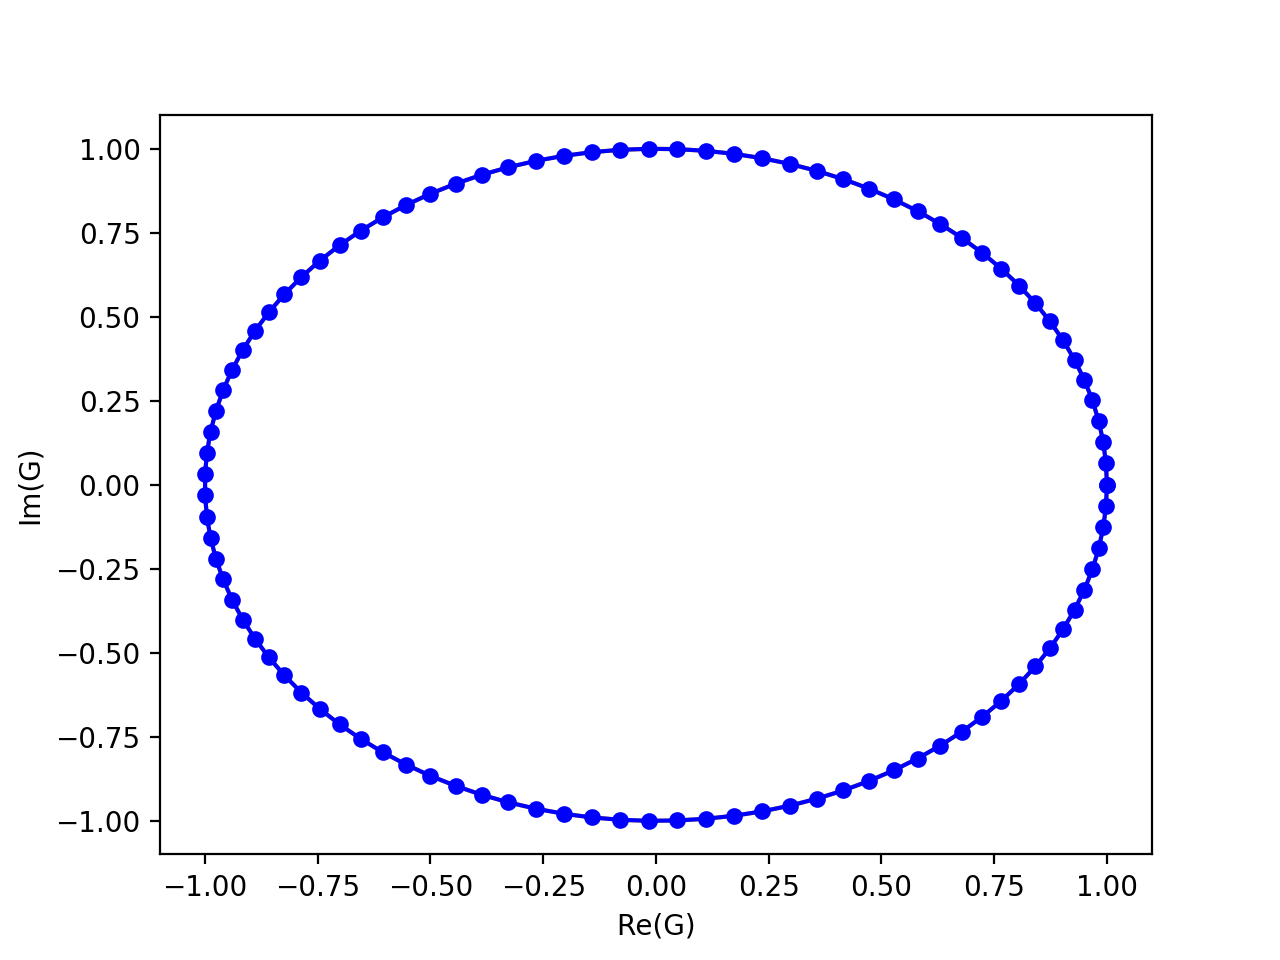
\includegraphics[width=10cm]{fig/vn10.png}
	\caption{Von–Neumann analysis with convection number = 1.0.} 
\end{figure}


\begin{figure}[H]
	\centering
	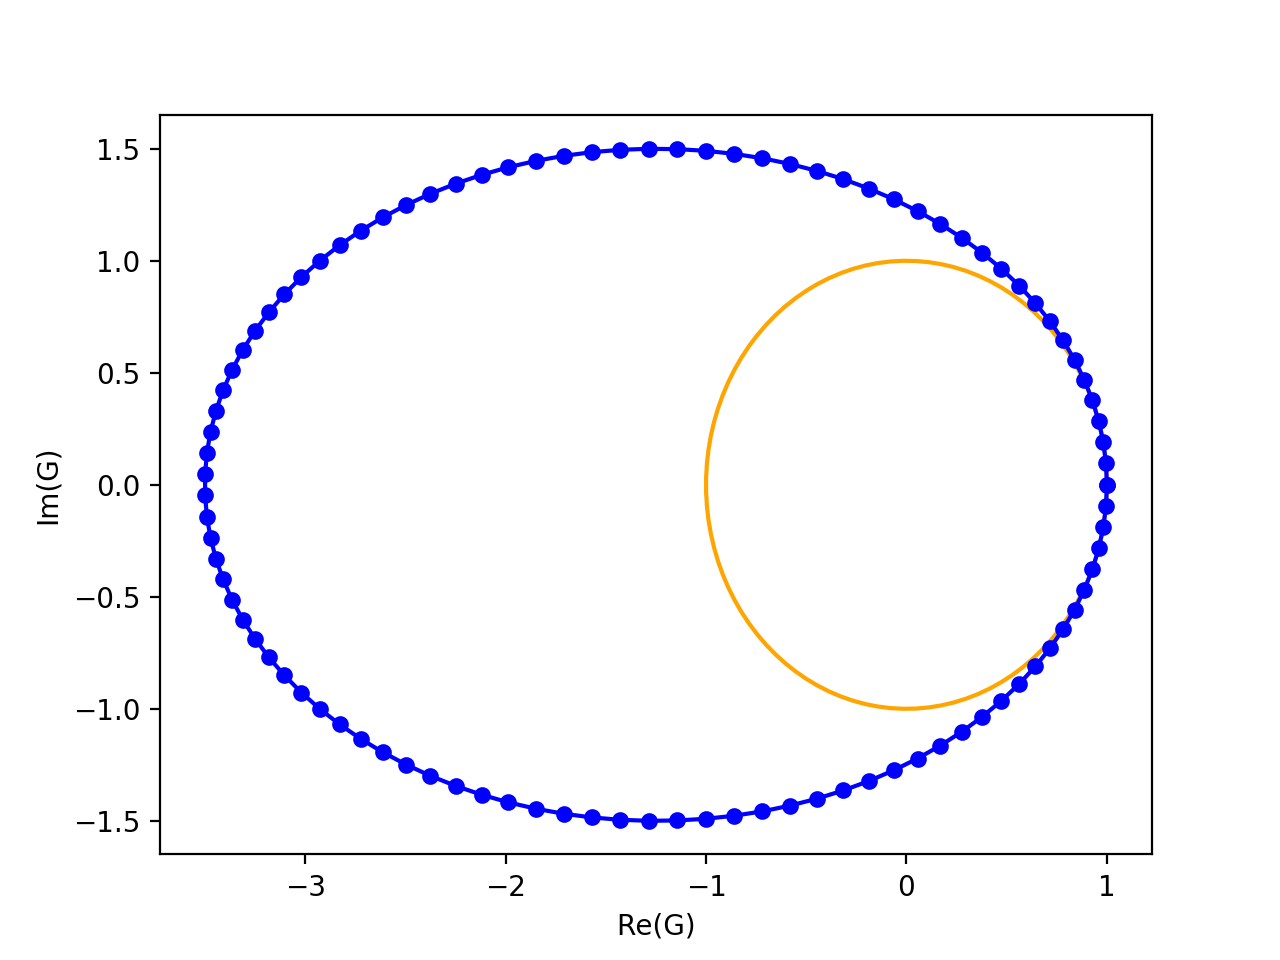
\includegraphics[width=10cm]{fig/vn15.png}
	\caption{Von–Neumann analysis with convection number = 1.5.} 
\end{figure}

\section{Time variation of convection with Lax–Wendroff scheme.}
I set convection number $c = 0.5$, mode number (number of waves) $m = 5$.
The results are shown below as Figure 4–6.

\begin{figure}[H]
	\centering
	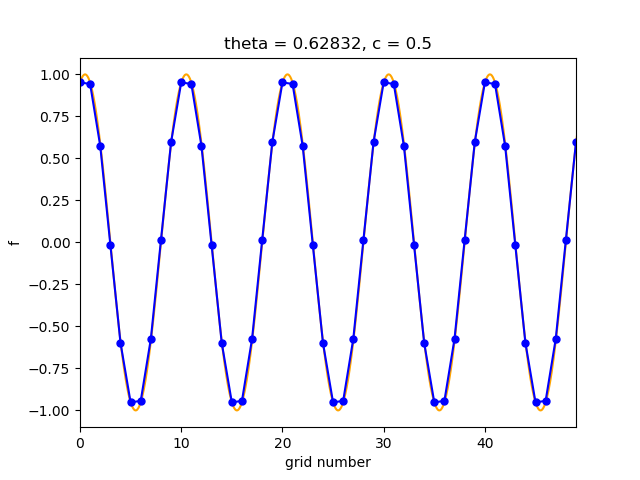
\includegraphics[width=10cm]{fig/lax_wen001}
	\caption{Lax–Wendroff time variation (iteration = 1).} 
\end{figure}


\begin{figure}[H]
	\centering
	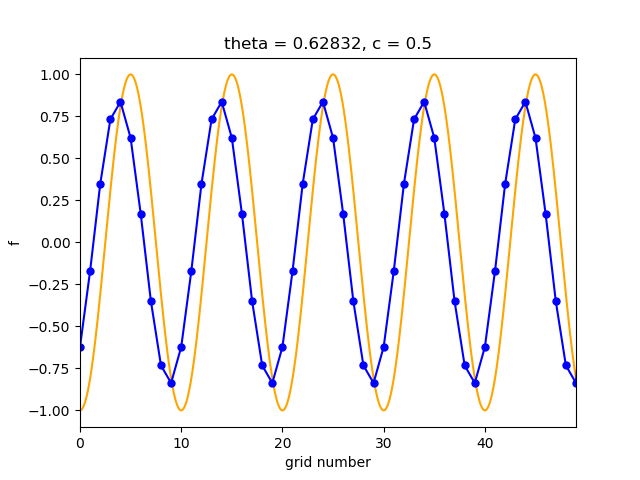
\includegraphics[width=10cm]{fig/lax_wen050}
	\caption{Lax–Wendroff time variation (iteration = 50).} 
\end{figure}

\begin{figure}[H]
	\centering
	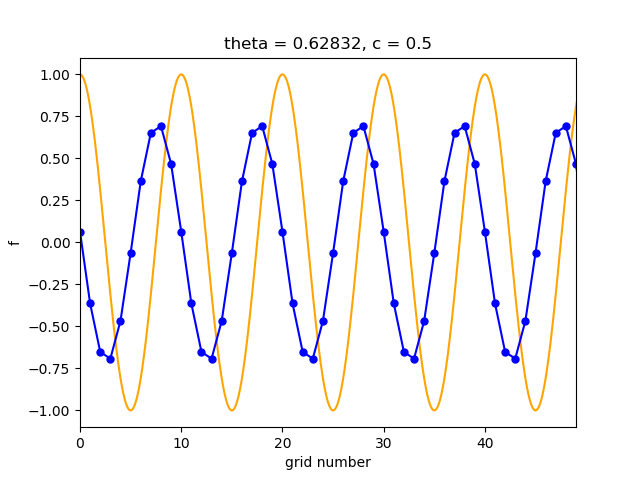
\includegraphics[width=10cm]{fig/lax_wen100}
	\caption{Lax–Wendroff time variation (iteration = 100).} 
\end{figure}


% END OF DOCUMENT
\end{document}
